\section{Tutorial -- Surrogates with the Flowsheet}\label{tutorial.surrogate.fs}

This section provides a brief tutorial for using the flowsheet plugin models generated by surrogate modeling methods. In the next FOQUS release all surrogate modeling methods will produce a model that can be run in a FOQUS flowsheet. \textbf{Currently iREVEAL does not produce a flowsheet model.}

\textbf{Before doing this tutorial complete the ALAMO tutorial in Section \ref{sec.surrogate.alamo}.}

\begin{enumerate}
	\item Open FOQUS.  If FOQUS has not been closed since completing the ALAMO tutorial, close it and reopen it. There is a known issue where existing flowsheet model plugins may not update until FOQUS is restarted.
	\item Enter ``FS\_Plugin\_Tutorial'' as the Session Name.
	\item Click the \bu{Flowsheet} button from the Home window.
	\item Click the \bu{Add Node} icon in the left toolbar (see Figure \ref{fig.pg.tut1}).
	\item Click a location for the node in the Flowsheet area.
	\item Enter ``model'' for the node name (without quotes).
	\item Click the \bu{Node Editor} icon in the left toolbar (see Figure \ref{fig.pg.tut1}).
	\item In the \textbf{\underline{Node Editor}}, select ``Plugin'' from the Model \textbf{\underline{Type}} drop-down list. 
	\item Select ``ALAMO\_Tutorial\_FS'' from the \textbf{\underline{Model}} drop-down list. 
	\item Set the \textbf{\underline{Value}} of the \textbf{\underline{Input Variables}} ``eq.x1'' to 2.
	\item Set the \textbf{\underline{Value}} of the \textbf{\underline{Input Variables}} ``eq.x2'' to 3.
	\item Click the \bu{Run} icon in the left toolbar (see Figure \ref{fig.pg.tut1}).
	\item Wait for the Flowsheet evaluation to complete. It should finish successfully.
	\item Check the value of the \textbf{\underline{Output Variables}}; the approximate values should be z1 = 5 and z2 = 13.
\end{enumerate}

\begin{figure}[H]
	\begin{center}
		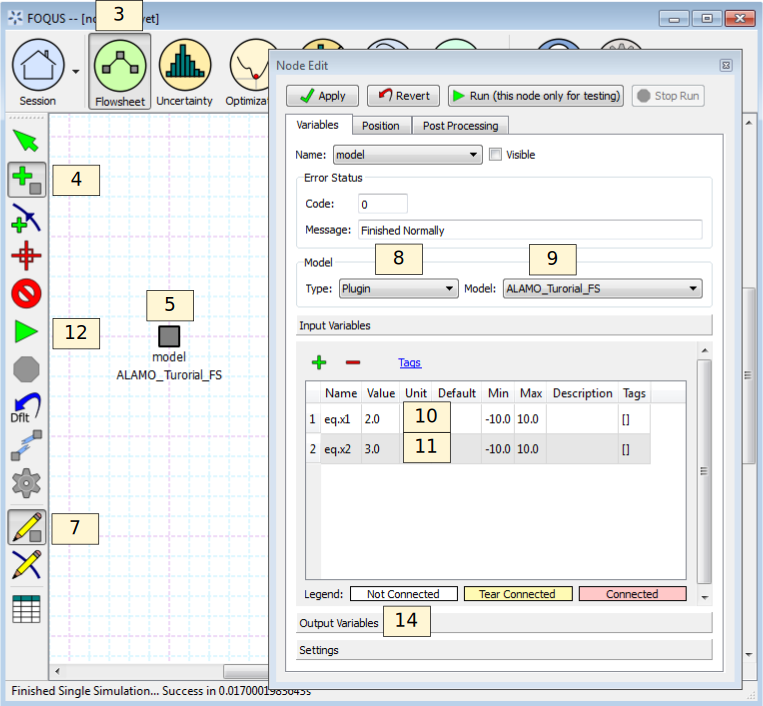
\includegraphics[scale=0.55]{Chapt_surrogates/figs/fs_plugin}
		\caption{Plugin Flowsheet}
		\label{fig.pg.tut1}
	\end{center}
\end{figure}
